\documentclass{beamer}
\usepackage{graphicx}
\usepackage{tabularx}
\usepackage{caption}
\usepackage{float}
\usepackage{anyfontsize}
\usepackage{multicol}
\usepackage[utf8]{inputenc}

\title{Mineração de dados aplicada à dados de evento no futebol}
\author{Luis Felipe Ramos \and Igor Lacerda Faria da Silva \and Matheus Tiago Pimenta de Souza}
\date{2024-07-28}

\captionsetup[figure]{labelformat=empty}% redefines the caption setup of the figures environment in the beamer class.

\begin{document}

\frame{\titlepage}

\begin{frame}
\frametitle{Uso de ciência de dados aplicada ao esporte}

\begin{columns}
\begin{column}{0.5\textwidth}
\centering
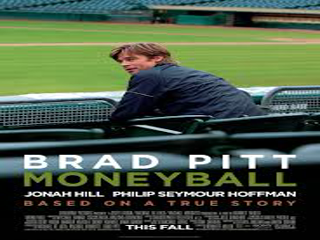
\includegraphics[width=\linewidth]{moneyball.png}
\captionof{figure}{Moneyball (2011)}
\end{column}
\begin{column}{0.5\textwidth}
\centering

\includegraphics[width=\linewidth]{fame.png}
\captionof{figure}{FAME}
\end{column}
\end{columns}
\end{frame}

\begin{frame}
\frametitle{Dados de súmula no futebol}
\begin{figure}[H]
\centering
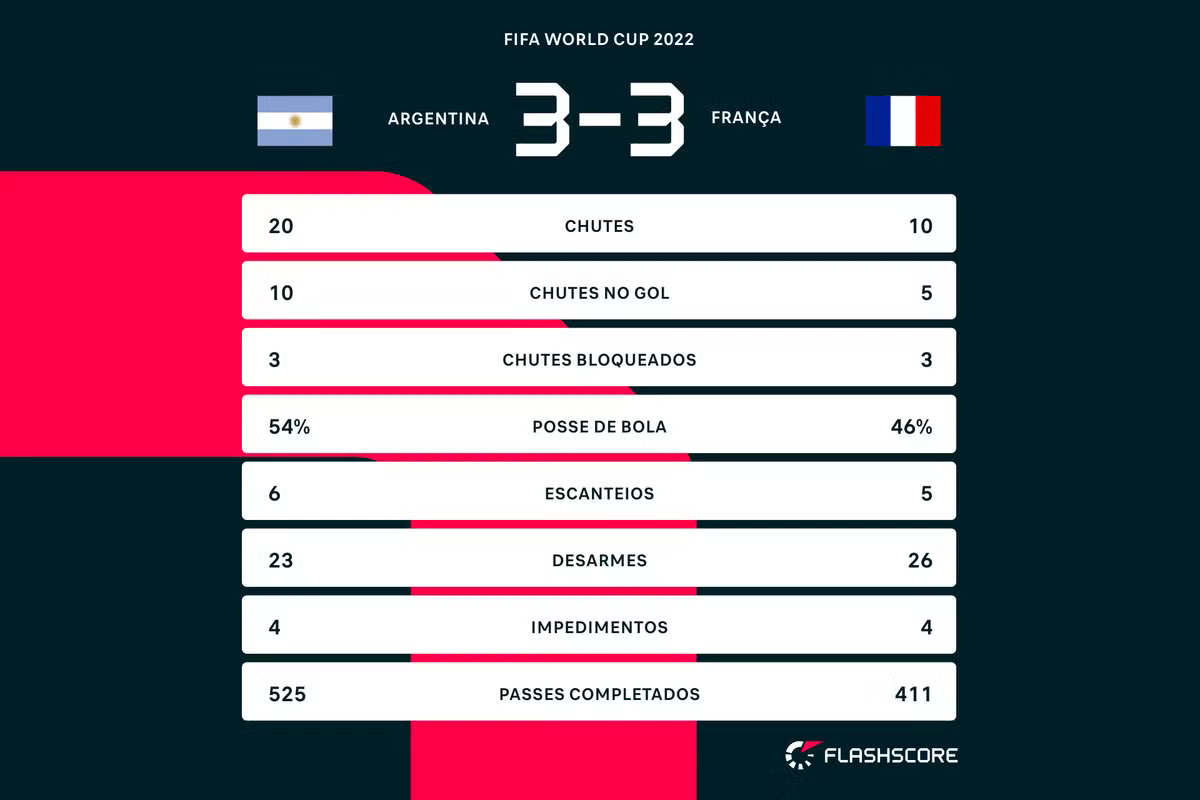
\includegraphics[width=\linewidth]{copa.jpg}
\caption{Estatísticas da final da Copa do Mundo de 2022}
\end{figure}
\end{frame}

\begin{frame}
\frametitle{Dados de evento}
\begin{figure}[H]
\centering
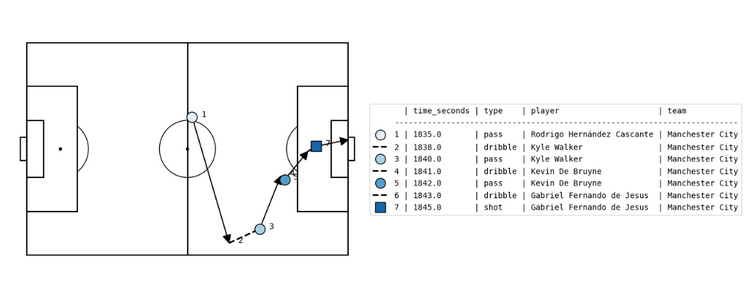
\includegraphics[width=\linewidth]{eventdatacity.png}
\caption{Jogada do Manchester City}
\end{figure}
\end{frame}

\begin{frame}
\frametitle{SPADL}
\begin{table}[H]
\centering
\begin{tabular}{|l|l|}
\hline
\textbf{Atributo} & \textbf{Descrição} \\
\hline
game\_id & O ID do jogo no qual a ação foi realizada \\
\hline
period\_id & O ID do período do jogo no qual a ação foi realizada \\
\hline
seconds & O tempo de início da ação \\
\hline
player & O jogador que realizou a ação \\
\hline
team & O time do jogador \\
\hline
start\_x & A localização x onde a ação começou \\
\hline
start\_y & A localização y onde a ação começou \\
\hline
end\_x & A localização x onde a ação terminou \\
\hline
end\_y & A localização y onde a ação terminou \\
\hline
action\_type & O tipo de ação (por exemplo, passe, chute, drible) \\
\hline
result & O resultado da ação (por exemplo, sucesso ou falha) \\
\hline
bodypart & A parte do corpo do jogador usada para a ação \\
\hline
\end{tabular}
\caption{Descrição dos dados no formato SPADL}
\end{table}
\end{frame}

\begin{frame}
    \frametitle{Distribuição dos tipos de ações}
\begin{figure}[H]
\centering
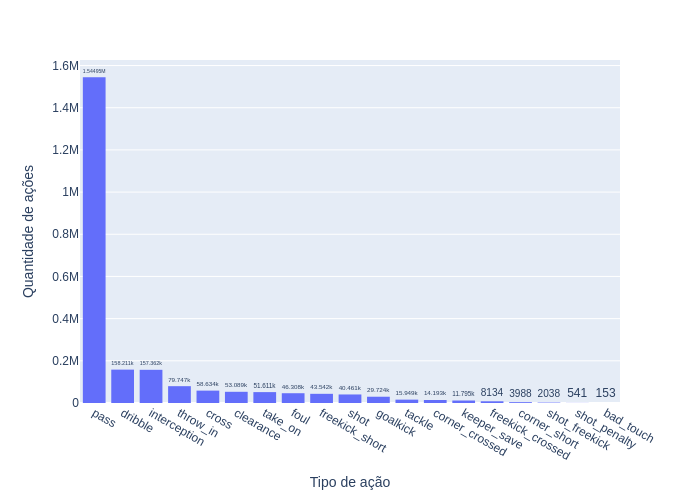
\includegraphics[width=\linewidth]{../report/images/action_distribution.png}
\end{figure}
\end{frame}

\begin{frame}
    \frametitle{Mapa de calor dos gols}
\begin{figure}[H]
\centering
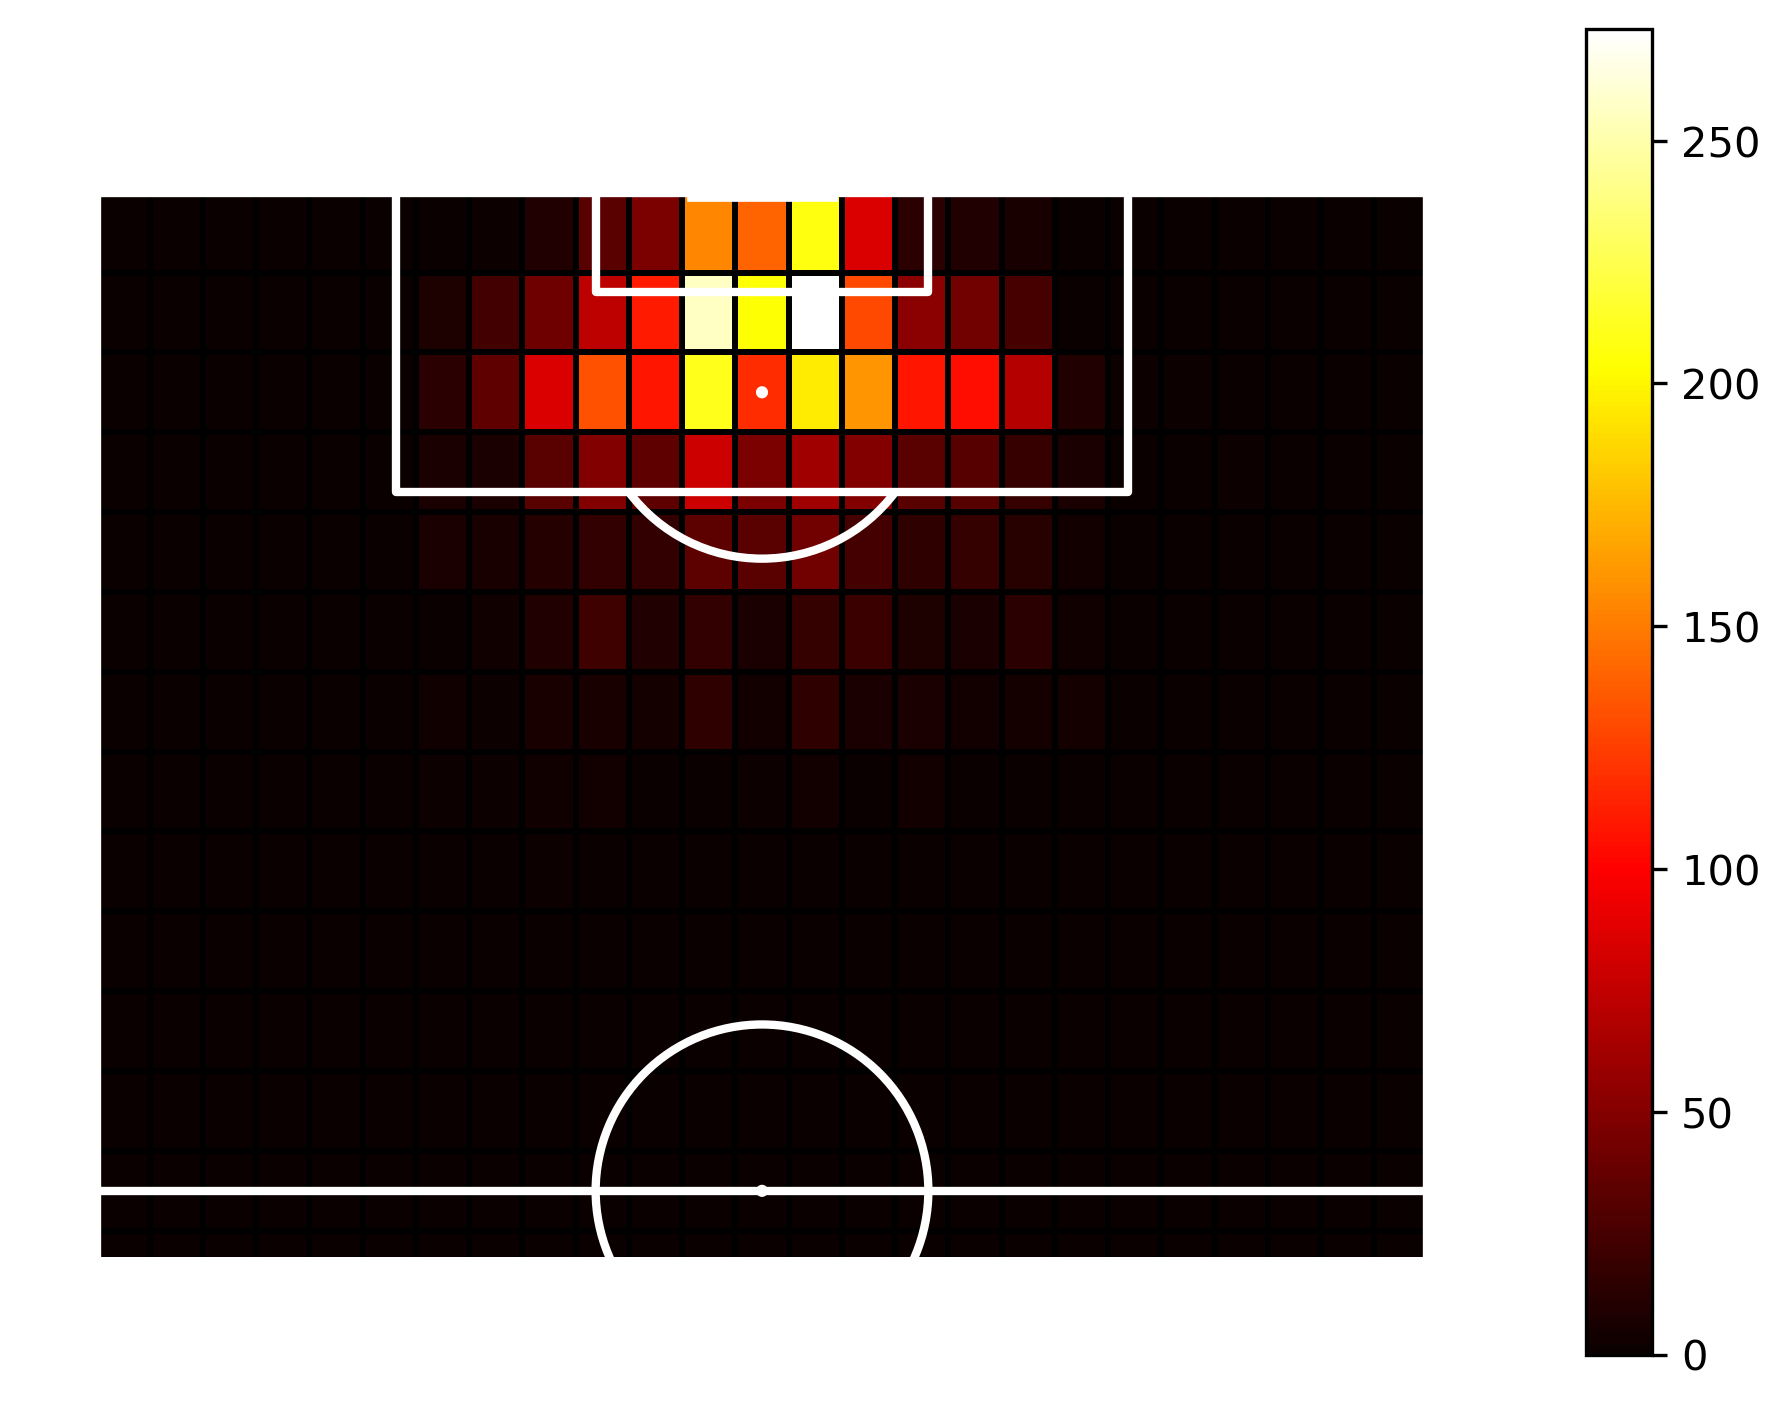
\includegraphics[width=\linewidth]{../report/images/goal_position_heatmap.png}
\end{figure}
\end{frame}

\begin{frame}
\frametitle{Objetivos}
\framesubtitle{Descoberta de subgrupos}
\begin{itemize}
    \item Trabalho motivador: \textit{Subgroup Discovery in Soccer Data}
    \item Reproduzir os experimentos do artigo e experimentar com novos alvos e um outro algoritmo de SD
\end{itemize}
\end{frame}

\begin{frame}
\frametitle{Objetivos}
\framesubtitle{Mineração de sequências}
\begin{itemize}
    \item Trabalho motivador: \textit{Supervised sequential pattern mining of event sequences in sport to identify important patterns of play: An application to rugby union}
    \item Aplicar as ideias em sequências de jogadas de futebol
\end{itemize}
\end{frame}

\begin{frame}
\frametitle{Gols Esperados (xG)}
\begin{itemize}
    \item Métrica de cálculo de probabilidade de gol
    \item Diferentes \textit{features} podem ser utilizadas:
    \begin{itemize}
        \item Distância para o gol
        \item Ângulo de chute
    \end{itemize}
\end{itemize}
\begin{figure}[H]
\centering
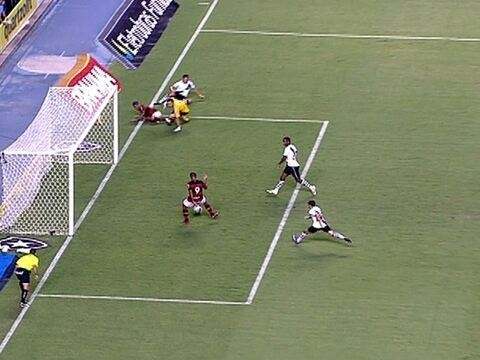
\includegraphics[width=\linewidth]{deivid.jpg}
\end{figure}
\end{frame}

\begin{frame}
\frametitle{VAEP}
\begin{itemize}
    \item Ações valem mais do que apenas gols
    \item O quanto cada jogada contribui para o aumento da chance de gol e diminiuição da chance de tomar gol?
\end{itemize}
\begin{figure}[H]
\centering
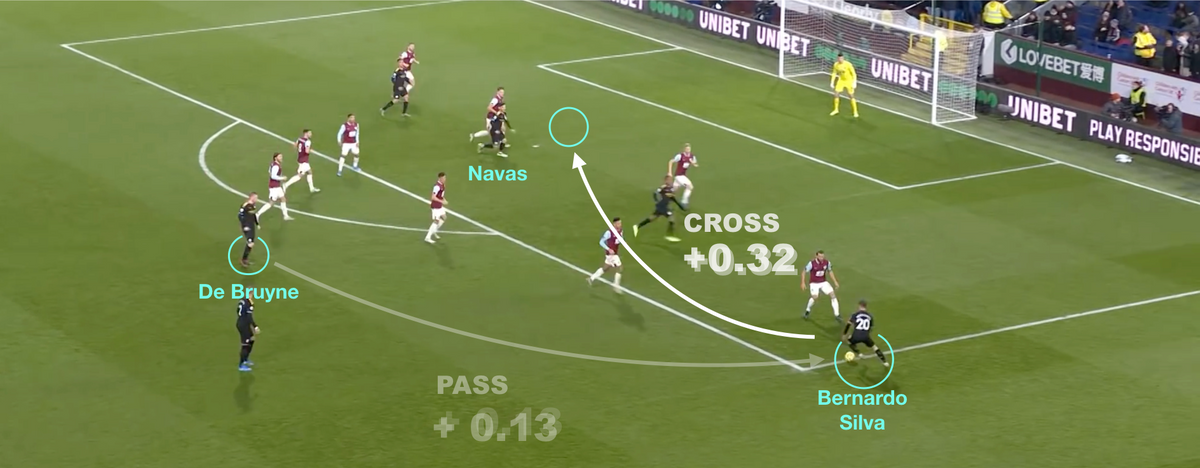
\includegraphics[width=\linewidth]{vaep.png}
\end{figure}
\end{frame}

\begin{frame}
\frametitle{Descoberta de subgrupos - Extração de \textit{Features}}
    \begin{table}[H]
        \centering
        \fontsize{6}{10}\selectfont % Definir tamanho da fonte específico
        \begin{tabularx}{\textwidth}{|l|X|}
            \hline
            \textbf{Atributo} & \textbf{Descrição} \\
            \hline
            start\_x & A localização x onde a ação começou \\
            \hline
            start\_y & A localização y onde a ação começou \\
            \hline
            num\_events & Contagem total de eventos (ações) na jogada \\
            \hline
            num\_passes & Contagem total de passes na jogada \\
            \hline
            num\_dribles & Contagem total de dribles na jogada \\
            \hline
            play\_duration & Duração total da jogada \\
            \hline
            player\_rank & Ranking do jogador \\
            \hline
            play\_distance & Distância (euclidiana) total percorrida na jogada \\
            \hline
            play\_mean\_distance\_to\_the\_goal & Distância (euclidiana) média de cada jogada até o gol \\
            \hline
            play\_std\_distance\_to\_the\_goal & Desvio padrão da distância (euclidiana) de cada jogada até o gol \\
            \hline
            play\_distance\_towards\_goal & Distância percorrida nas jogadas em direção ao gol (considerando só o eixo x) \\
            \hline
            bodypart\_name & A parte do corpo do jogador usada para a ação \\
            \hline
            ratio\_distance & Razão entre play\_distance e play\_distance\_towards\_goal \\
            \hline
            total\_time\_per\_play & Desvio padrão da distância (euclidiana) de cada jogada até o gol \\
            \hline
            play\_duration & Duração total das jogadas \\
            \hline
            total\_time\_per\_play & Média do tempo por jogada (razão entre play\_duration e num\_events) \\
            \hline
            play\_speed & Razão entre play\_distance e play\_duration \\
            \hline
            play\_speed\_towards\_goal & Razão entre play\_distance\_towards\_goal e play\_duration \\
            \hline
        \end{tabularx}
        \label{tab:atributosSD}
    \end{table}
\end{frame}

\begin{frame}
\frametitle{Descoberta de subgrupos - Estratégias}
\begin{itemize}
    \item Avaliações em 3 tipos de granularidades
    \begin{itemize}
        \item Avaliação de Todo o Dasatet VS Duas ligas diferentes
        \item Avaliação de três times de uma mesma liga (1º, 10º e 20°) 
        \item Avaliação de duas abordagens de SD (Beam Search e SSD++)
    \end{itemize}
\end{itemize}
\begin{itemize}
    \item Todas as avaliações nos três alvos (Gol/Não Gol, xG e VAEP)
    \item As duas primeiras avaliações com Beam Search do pacote do \textit{pysubgroup}, 
    com profundidade 3, buscando 100 subgrupos com largura do Beam de 250
    \item \textit{SSD++} com profundidade 3, largura do beam de 25 e máximo de regras sendo 20
\end{itemize}
\end{frame}

\begin{frame}
\frametitle{Descoberta de subgrupos - Resultados Métricas}
    \begin{table}[H]
        \centering
        \fontsize{6}{10}\selectfont % Definir tamanho da fonte específico
        \begin{tabular}{|l|l|l|l|l|}
            \hline
            \textbf{Algoritmo} & \textbf{Dado} &  \textbf{Target} & 
            \textbf{WRAcc do melhor} & \textbf{Cobertura Total}
            \\
            \hline
            Beam Search & Todo dataset & Gol & 0.0312 & 0.5099 
            \\
            \hline
            Beam Search & Todo dataset & xG & 0.0187 & 0.5046 
            \\
            \hline
            Beam Search & Todo dataset & VAEP & 0.0307 & 0.5099 
            \\
            \hline
            Beam Search & Inglaterra & Gol & 0.03192 & 0.4980 
            \\
            \hline
            Beam Search & Inglaterra & xG & 0.0203 & 0.4933 
            \\
            \hline
            Beam Search & Inglaterra & VAEP & 0.0317 & 0.4977
            \\
            \hline
            Beam Search & Espanha & Gol & 0.0307 & 0.5110 
            \\
            \hline
            Beam Search & Espanha & xG & 0.0195 & 0.3983 
            \\
            \hline
            Beam Search & Espanha & VAEP & 0.0304 & 0.5120 
            \\
            \hline
            Beam Search & Man City & Gol & 0.0483 & 0.5721 
            \\
            \hline
            Beam Search & Man City & xG & 0.0303 & 0.4959 
            \\
            \hline
            Beam Search & Man City & VAEP & 0.0487 & 0.5656 
            \\
            \hline
            Beam Search & Newcastle & Gol & 0.0405 & 0.6561 
            \\
            \hline
            Beam Search & Newcastle & xG & 0.0247 & 0.3878 
            \\
            \hline
            Beam Search & Newcastle & VAEP & 0.0420 & 0.6561 
            \\
            \hline
            Beam Search & West Bromwich & Gol & 0.0293 & 0.5499 
            \\
            \hline
            Beam Search & West Bromwich & xG & 0.0307 & 0.3989 
            \\
            \hline
            Beam Search & West Bromwich & VAEP & 0.0287 & 0.5254 
            \\
            \hline
            SSD++ & Todo Dataset & Gol & 0.0164 & 0.7818 
            \\
            \hline
            SSD++ & Todo Dataset & xG & 0.0117 & 0.9956
            \\
            \hline
            SSD++ & Todo Dataset & VAEP & 0.0194 & 0.8114
            \\
            \hline
        \end{tabular}
        \label{tab:resultMetricas}
    \end{table}
\end{frame}

\begin{frame}
\frametitle{Descoberta de subgrupos - Resultados entre Ligas}
\begin{table}[H]
    \centering
    \fontsize{6}{10}\selectfont % Definir tamanho da fonte específico
    \begin{tabularx}{\textwidth}{|l|l|X|}
        \hline
        \textbf{Dataset} & \textbf{Target} & \textbf{Subgrupo} \\
        \hline
        Todo dataset & Gol & $ \text{shot\_angle\_from\_goal} \geq 0.60 \ \text{AND} \ \text{shot\_distance\_from\_goal} < 11.26 $ \\
        \hline
        Todo dataset & xG & $ \text{shot\_angle\_from\_goal} \geq 0.60 \ \text{AND} \ \text{shot\_distance\_from\_goal} < 11.26 \ \text{AND} \ \text{start\_x} \geq 96.60 $ \\
        \hline
        Todo dataset & VAEP & $ \text{num\_dribbles} : [0:1[ \ \text{AND} \ \text{shot\_angle\_from\_goal} \geq 0.60 \ \text{AND} \ \text{shot\_distance\_from\_goal} < 11.26 $ \\
        \hline
        Inglaterra & Gol & $ \text{shot\_angle\_from\_goal} \geq 0.61 \ \text{AND} \ \text{shot\_distance\_from\_goal} < 11.26 $ \\
        \hline
        Inglaterra & xG & $ \text{num\_dribbles} : [0:1[ \ \text{AND} \ \text{shot\_distance\_from\_goal} < 11.26 \ \text{AND} \ \text{start\_x} \geq 96.60 $ \\
        \hline
        Inglaterra & VAEP & $ \text{play\_duration} < 1.39 \ \text{AND} \ \text{shot\_distance\_from\_goal} < 11.26 \ \text{AND} \ \text{total\_time\_per\_play} < 0.65 $ \\
        \hline
        Espanha & Gol & $ \text{shot\_angle\_from\_goal} \geq 0.61 \ \text{AND} \ \text{shot\_distance\_from\_goal} < 11.04 \ \text{AND} \ \text{start\_x} \geq 96.60 $ \\
        \hline
        Espanha & xG & $ \text{shot\_angle\_from\_goal} \geq 0.61 $ \\
        \hline
        Espanha & VAEP & $ \text{play\_distance\_towards\_goal} : [0.0:7.35[ \ \text{AND} \ \text{ratio\_distance} : [0.0:0.12[ \ \text{AND} \ \text{shot\_distance\_from\_goal} < 11.04 $ \\
        \hline
    \end{tabularx}
    \label{tab:resultsSD}
\end{table}
\end{frame}

\begin{frame}
\frametitle{Descoberta de subgrupos - Resultados entre Times}
    \begin{table}[H]
        \centering
        \fontsize{6}{10}\selectfont % Definir tamanho da fonte específico
        \begin{tabularx}{\textwidth}{|l|l|X|}
            \hline
            \textbf{Dataset} & \textbf{Target} & \textbf{Subgrupo} \\
            \hline
            Man City & Gol & $ \text{player\_rank} : [0.02:0.03[ \ \text{AND} \ \text{shot\_distance\_from\_goal} < 10.90 \ \text{AND} \ \text{start\_x} > 96.60 $ \\
            \hline
            Man City & xG & $ \text{num\_dribbles} : [0:2[ \ \text{AND} \ \text{shot\_angle\_from\_goal} \geq 0.62 \ \text{AND} \ \text{start\_x} \geq 96.60 $ \\
            \hline
            Man City & VAEP & $ \text{bodypart\_name} = \text{foot\_left} \ \text{AND} \ \text{shot\_distance\_from\_goal} < 11.03 $ \\
            \hline
            Newcastle & Gol & $ \text{shot\_angle\_from\_goal} \geq 0.61 \ \text{AND} \ \text{shot\_distance\_from\_goal} < 11.04 $ \\
            \hline
            Newcastle & xG & $ \text{num\_dribbles} : [1:3[ \ \text{AND} \ \text{start\_x} \geq 96.60 \ \text{AND} \ \text{start\_y} : [33.32:38.08[ $ \\
            \hline
            Newcastle & VAEP & $ \text{bodypart\_name} = \text{foot\_right} \ \text{AND} \ \text{shot\_distance\_from\_goal} < 11.04 $ \\
            \hline
            West Bromwich & Gol & $ \text{bodypart\_name} = \text{head/other} \ \text{AND} \ \text{shot\_distance\_from\_goal} < 10.52 \ \text{AND} \ \text{start\_x} \geq 96.60 $ \\
            \hline
            West Bromwich & xG & $ \text{num\_dribbles} : [0:2[ \ \text{AND} \ \text{start\_x} \geq 96.60 $ \\
            \hline
            West Bromwich & VAEP & $ \text{bodypart\_name} = \text{head/other} \ \text{AND} \ \text{play\_distance\_towards\_goal} : [39.90:56.70[ \ \text{AND} \ \text{start\_x} \geq 96.60 $ \\
            \hline
        \end{tabularx}
    \end{table}
\end{frame}

\begin{frame}
\frametitle{Descoberta de subgrupos - Resultados entre Algoritmos}
    \begin{table}[H]
        \centering
        \fontsize{6}{10}\selectfont % Definir tamanho da fonte específico
        \begin{tabularx}{\textwidth}{|l|l|X|}
            \hline
            \textbf{Dataset} & \textbf{Target} & \textbf{Subgrupo} \\
            \hline
            BS & Gol & $ \text{start\_x} \geq 96.60 $ \\
            \hline
            BS & Gol & $ \text{num\_dribbles} : [0:1[ \text{ AND } \text{shot\_angle\_from\_goal} \geq 0.60 \text{ AND } \text{shot\_distance\_from\_goal} < 11.26 $ \\
            \hline
            BS & xG & $ \text{start\_x} \geq 96.60 \text{ AND } \text{start\_y} : [31.96:37.40[ $ \\
            \hline
            BS & xG & $ \text{shot\_angle\_from\_goal} \geq 0.60 \text{ AND } \text{shot\_distance\_from\_goal} < 11.26 $ \\
            \hline
            BS & VAEP & $ \text{start\_x} \geq 96.60 $ \\
            \hline
            BS & VAEP & $ \text{num\_dribbles} : [0:1[ \text{ AND } \text{shot\_distance\_from\_goal} < 11.26 $ \\
            \hline
            SSD++ & Gol & $ \text{shot\_angle\_from\_goal} \geq 0.5591 \text{ AND } \text{bodypart\_name} = \text{foot\_right} \text{ AND } \text{start\_x} \geq 95.55 $ \\
            \hline
            SSD++ & Gol & $ \text{player\_rank} \geq 0.016 \text{ AND } 2.0 \leq \text{num\_passes} \leq 3.0 \text{ AND } 0.359 \leq \text{shot\_angle\_from\_goal} \leq 0.5591 $ \\
            \hline
            SSD++ & xG & $ 27.2 \leq \text{start\_y} \leq 34.0 \text{ AND } 4.64 \leq \text{play\_speed} \leq 6.87 \text{ AND } \text{num\_dribbles} \geq 1.0 $ \\
            \hline
            SSD++ & xG & $ \text{play\_speed} \geq 8.98 \text{ AND } \text{play\_duration} \geq 2.07 \text{ AND } 0.004 \leq \text{player\_rank} \leq 0.016 $ \\
            \hline
            SSD++ & VAEP & $ \text{shot\_angle\_from\_goal} \geq 0.56 \text{ AND } 0.004 \leq \text{player\_rank} \leq 0.016 \text{ AND } 0.93 \leq \text{total\_time\_per\_play} \leq 1.76 $ \\
            \hline
            SSD++ & VAEP & $ \text{shot\_angle\_from\_goal} \geq 0.56 \text{ AND } \text{play\_speed\_towards\_goal} \geq 1.52 \text{ AND } 12.39 \leq \text{play\_mean\_distance\_to\_the\_goal} \leq 28.09 $ \\
            \hline
        \end{tabularx}
        \label{tab:resultAlgoritms}
    \end{table}
\end{frame}

\begin{frame}
\frametitle{Descoberta de subgrupos - Conclusões}
\begin{itemize}
    \item Alvos
    \begin{itemize}
        \item VAEP se mostrou coerente com xG e Gol/Não Gol
        \item xG levou a métricas menores, mas grupos são parecidos
        \item Nenhuma métrica se sobressaiu
    \end{itemize}
    \item Algoritmos
    \begin{itemize}
        \item Beam Search com maior WRAcc, mas menor cobertura
        \item Acreditamos que os resultados são complementares
    \end{itemize}
    \item Utilidade dos padrões
    \begin{itemize}
        \item Beam Search mais simples, úteis para compara times
        \item SSD++ mais diferentes, permitindo análises mais exóticas
    \end{itemize}
\end{itemize}
\end{frame}

\begin{frame}
\frametitle{Mineração de Sequências}
    \begin{itemize}
        \item Resultados não muito promissores usando o SPP
    \end{itemize}
    \begin{center}
        \begin{tabular}{|c|c|}
            \hline
            \textbf{Métrica} & \textbf{Sequência} \\
            \hline
            xG & pass pass pass cross drible  \\
            \hline
            Binário & pass pass drible pass drible \\
            \hline
            VAEP & pass pass pass drible take on \\
            \hline
        \end{tabular}
    \end{center}
\end{frame}

\begin{frame}
\frametitle{Fim}
\begin{itemize}
    \item Perguntas, comentários, etc 
\end{itemize}
\end{frame}

\end{document}

